\hypertarget{_clip_8cpp}{
\section{Clip.cpp File Reference}
\label{_clip_8cpp}\index{Clip.cpp(125)@{Clip.cpp(125)}}
}


\subsection{Detailed Description}
Implementation of class \hyperlink{class_clip}{Clip}. 



Definition in file \hyperlink{_clip_8cpp-source}{Clip.cpp}.

{\tt \#include \char`\"{}Clip.h\char`\"{}}\par
{\tt \#include \char`\"{}NessieException.h\char`\"{}}\par
{\tt \#include $<$iostream$>$}\par
{\tt \#include $<$Magick++.h$>$}\par


Include dependency graph for Clip.cpp:\nopagebreak
\begin{figure}[H]
\begin{center}
\leavevmode
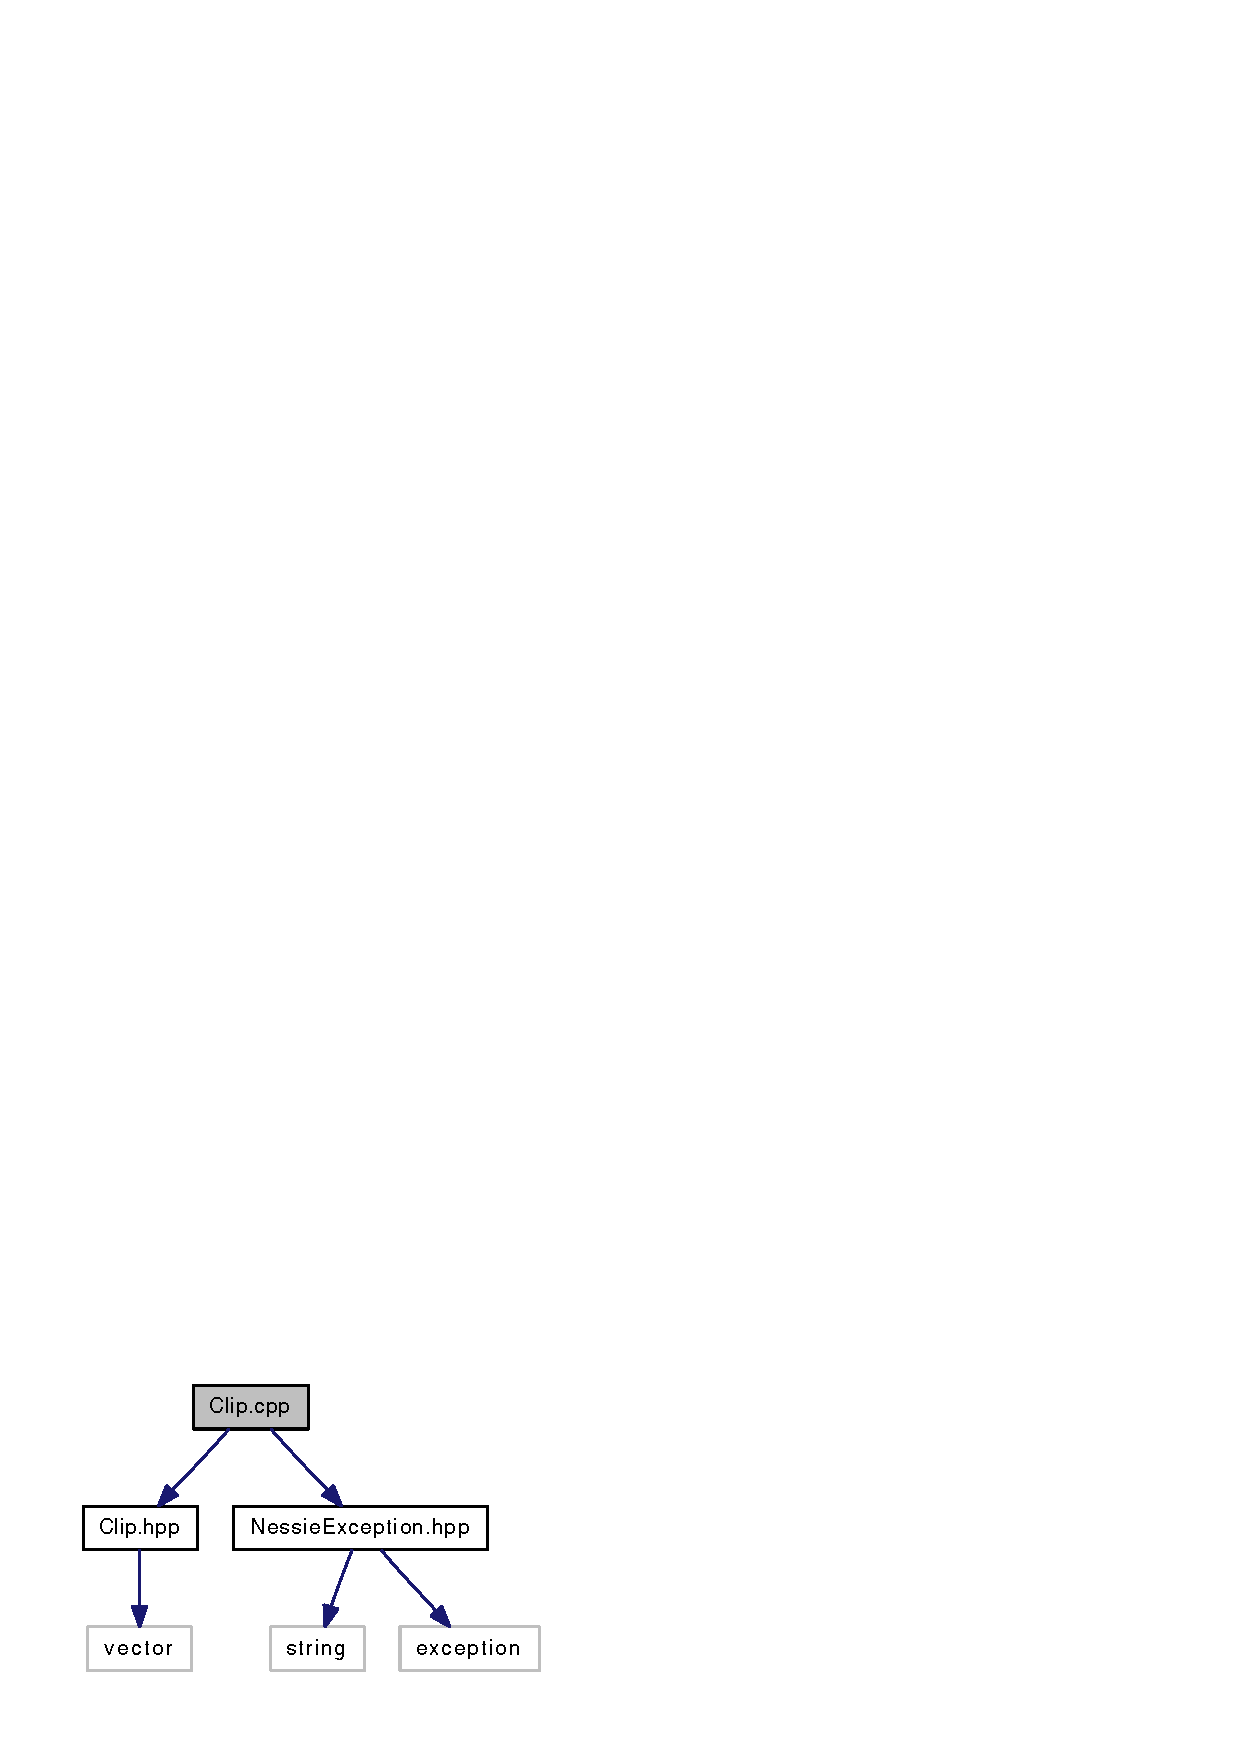
\includegraphics[width=181pt]{_clip_8cpp__incl}
\end{center}
\end{figure}
